\section{Stopped Kaon}
\label{Sec:Kaon}
\begin{itemize}
\item Stopping point of the Kaon is identified as kink of the track
\item For example, $K\to\mu\nu$ event (Fig.~\ref{Fig:SimulatedKaon}) is composed by two tracks, Kaon and muon, and intersection of two tracks corresponds to the stopped point.
\item We develop two different algorithm to identify the Kaon stopped point, Hough and Chi2.
\end{itemize}

Hough transform was invented for machine analysis of bubble chamber photographs by Paul.V.C.Hough.\cite{3069654}.
\begin{itemize}
\item Transform hit coordinates [TPC channel, drift time] into Hough space
\item Find the straight line by choosing the most dense point in Hough space (= Kaon track)
\item Hits associated with the first straight line are removed, and remaining hit coordinates are transformed into Hough space.
\item Find second straight line using the same procedure ( = Muon track)
\item This procedure is repeated until number of remaining hits are less than three.
\item Kaon stopped point is identified as the hit with maximum charge and around the intersection of two lines.
\end{itemize}

%Figure \ref{hmap2} shows hit map like a Kaon track.
%One point in the X-Y space can be transformed into sinusoidal curve in the $\rho$-$\theta$ space.Figure \ref{rho_theta2} shows sinusoidal curves in all points.
%And, we find the straight line associated with the largest number of points by choosing the most dense point in $\rho$-$\theta$ space.
%Next , the sinusoidal curves of the hits associated with frist straight line are removed from figure \ref{rho_theta2}.
%Figure \ref{rho_theta3} shows sinusoidal curves after the hits associated with frist straight line removed.
%We find second straight line using the same procedure.This procedure is repeated until there are less than three points.
%Figure \ref{hmap_fit} shows the two straight lines found by hough transform mehotd.\\
%Kaon stopped point in the liquid argon detecor defined as charge maximum point around the intersection of some lines.

%\begin{figure}[!htb]
%  \begin{minipage}{0.5\hsize}
%    \begin{center}
%      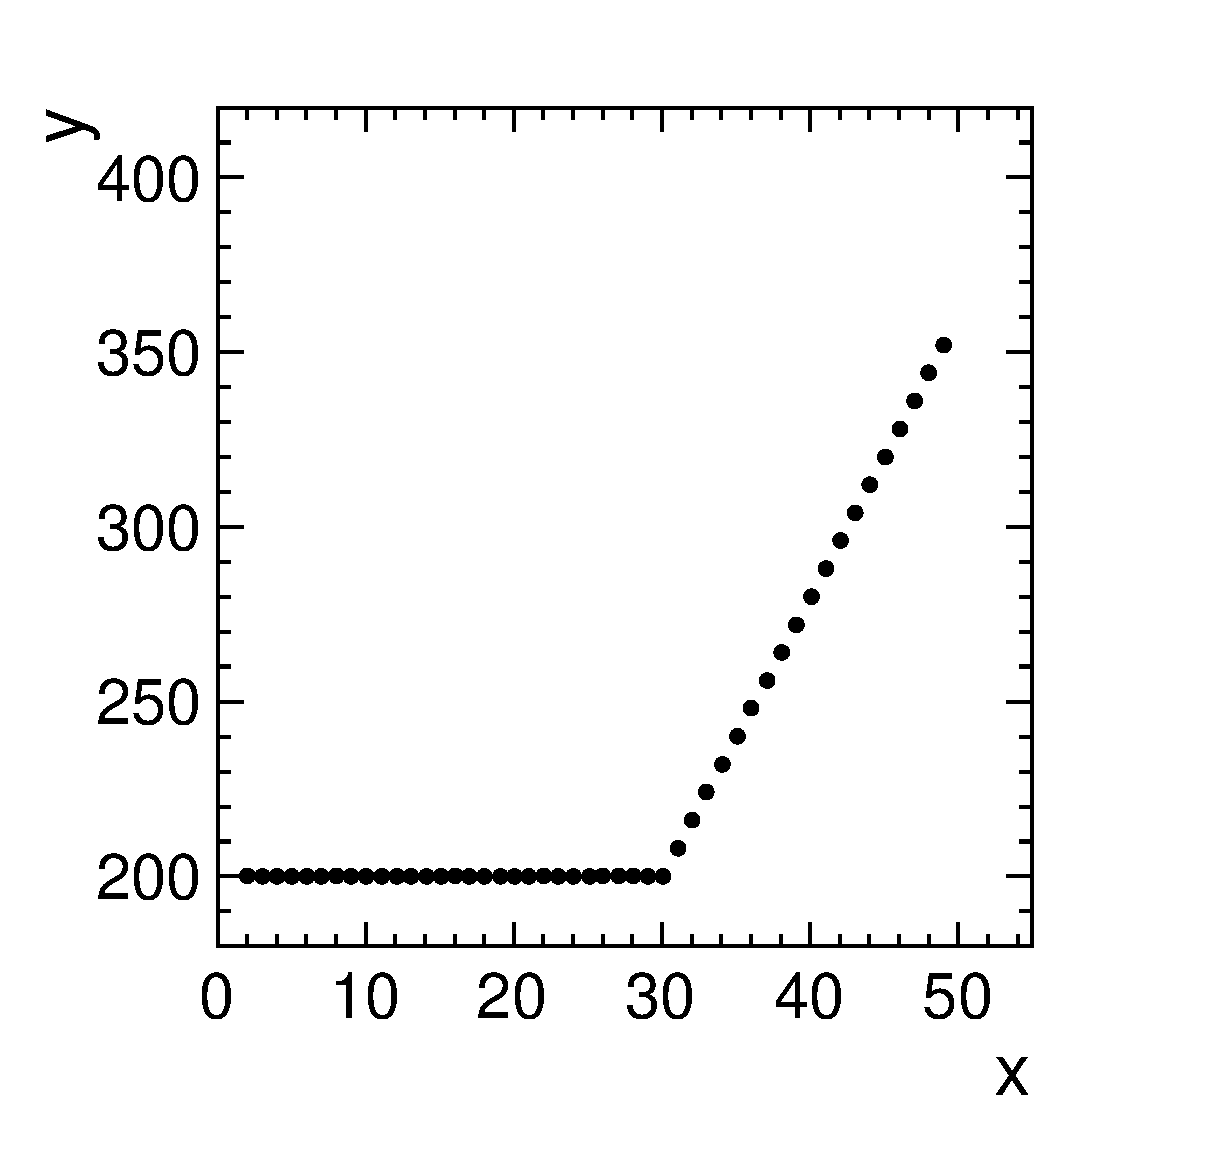
\includegraphics[width=35mm]{fig/hmap2.eps}
%    \end{center}
%    \caption{Hit map like a Kaon track}
%    \label{hmap2}
%  \end{minipage}
%  \begin{minipage}{0.5\hsize}
%    \begin{center}
%      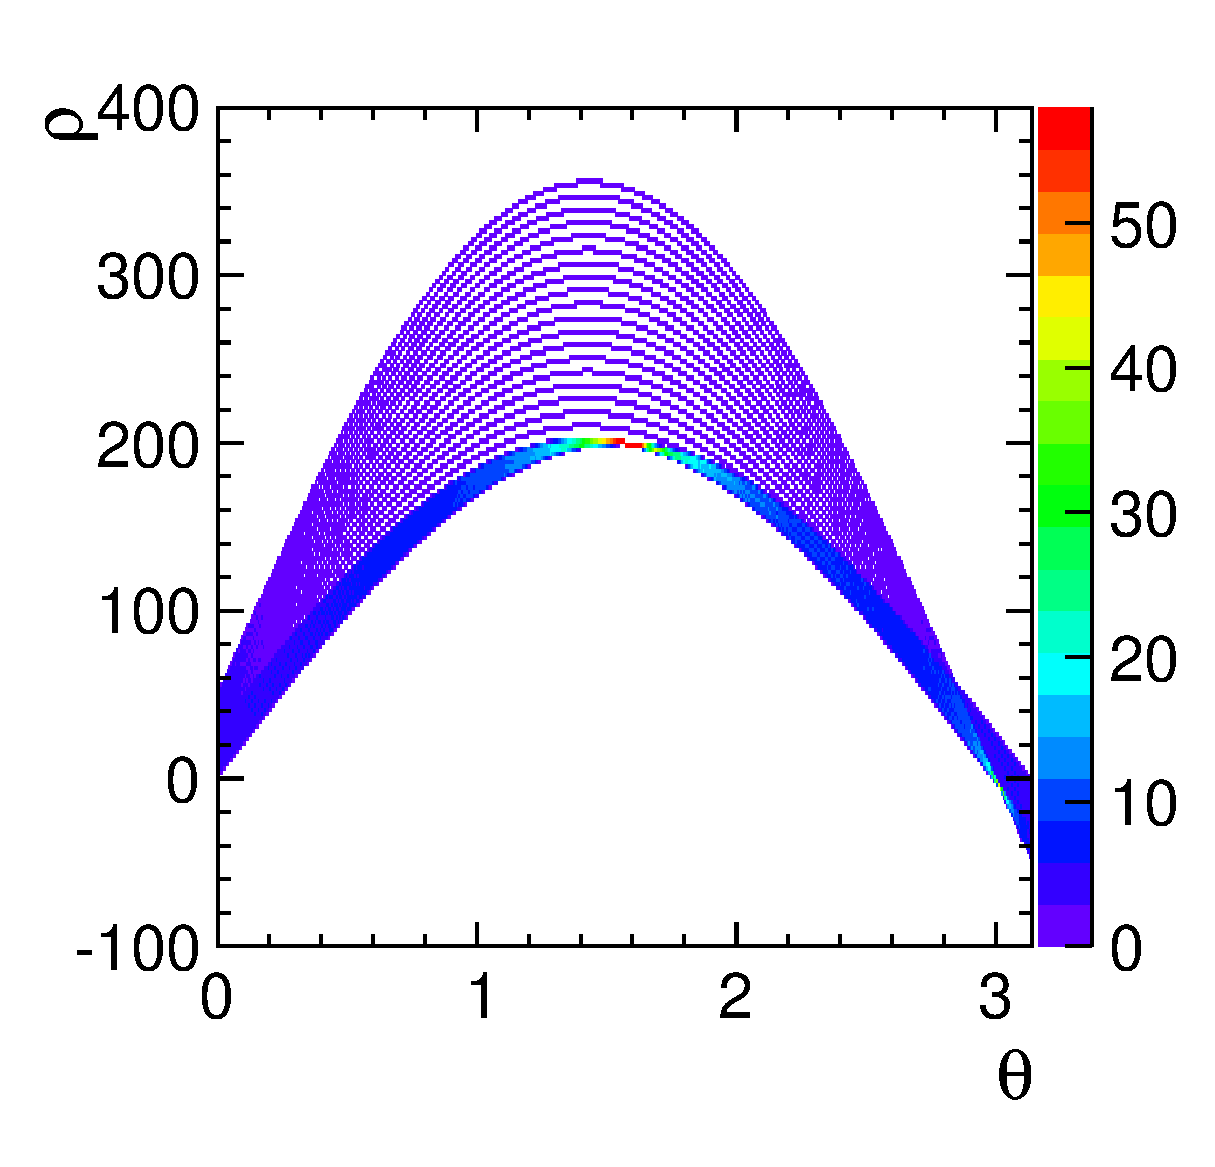
\includegraphics[width=35mm]{fig/rho_theta2.eps}
%    \end{center}
%    \caption{sinusoidal curves getting form all hough transformed  points of Figure \ref{hmap2}}
%    \label{rho_theta2}
%  \end{minipage}
%  \\
%  \begin{minipage}{0.5\hsize}
%    \begin{center}
%      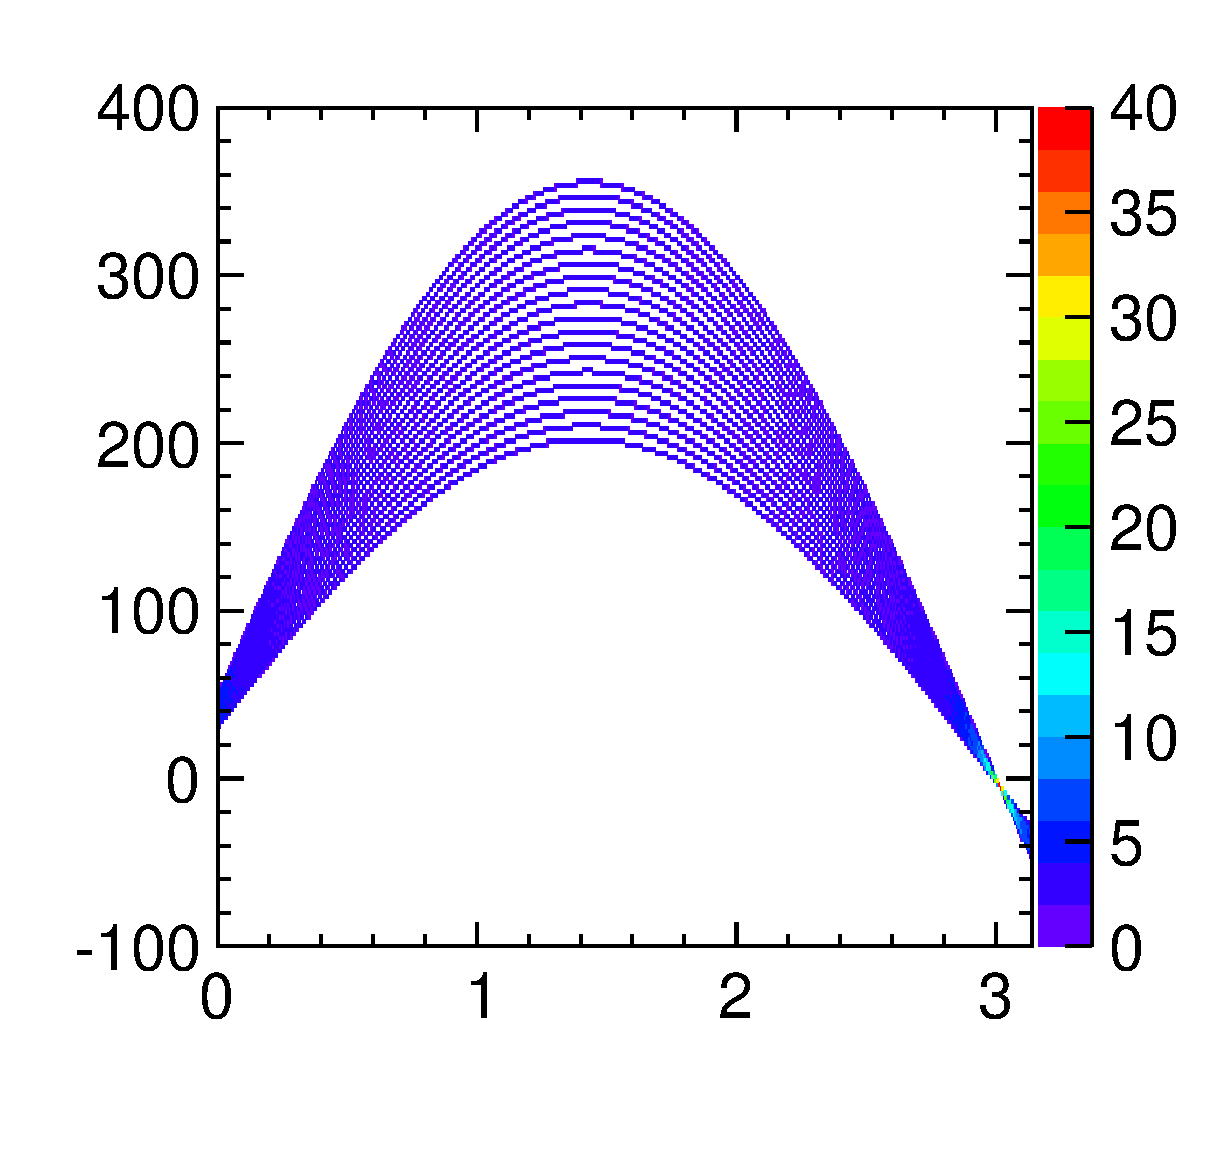
\includegraphics[width=35mm]{fig/rho_theta_kink.eps}
%    \end{center}
%    \caption{sinusoidal curves removed the points associated with first straight line from figure \ref{rho_theta2}}
%    \label{rho_theta3}
%  \end{minipage}
%  \begin{minipage}{0.5\hsize}
%    \begin{center}
%      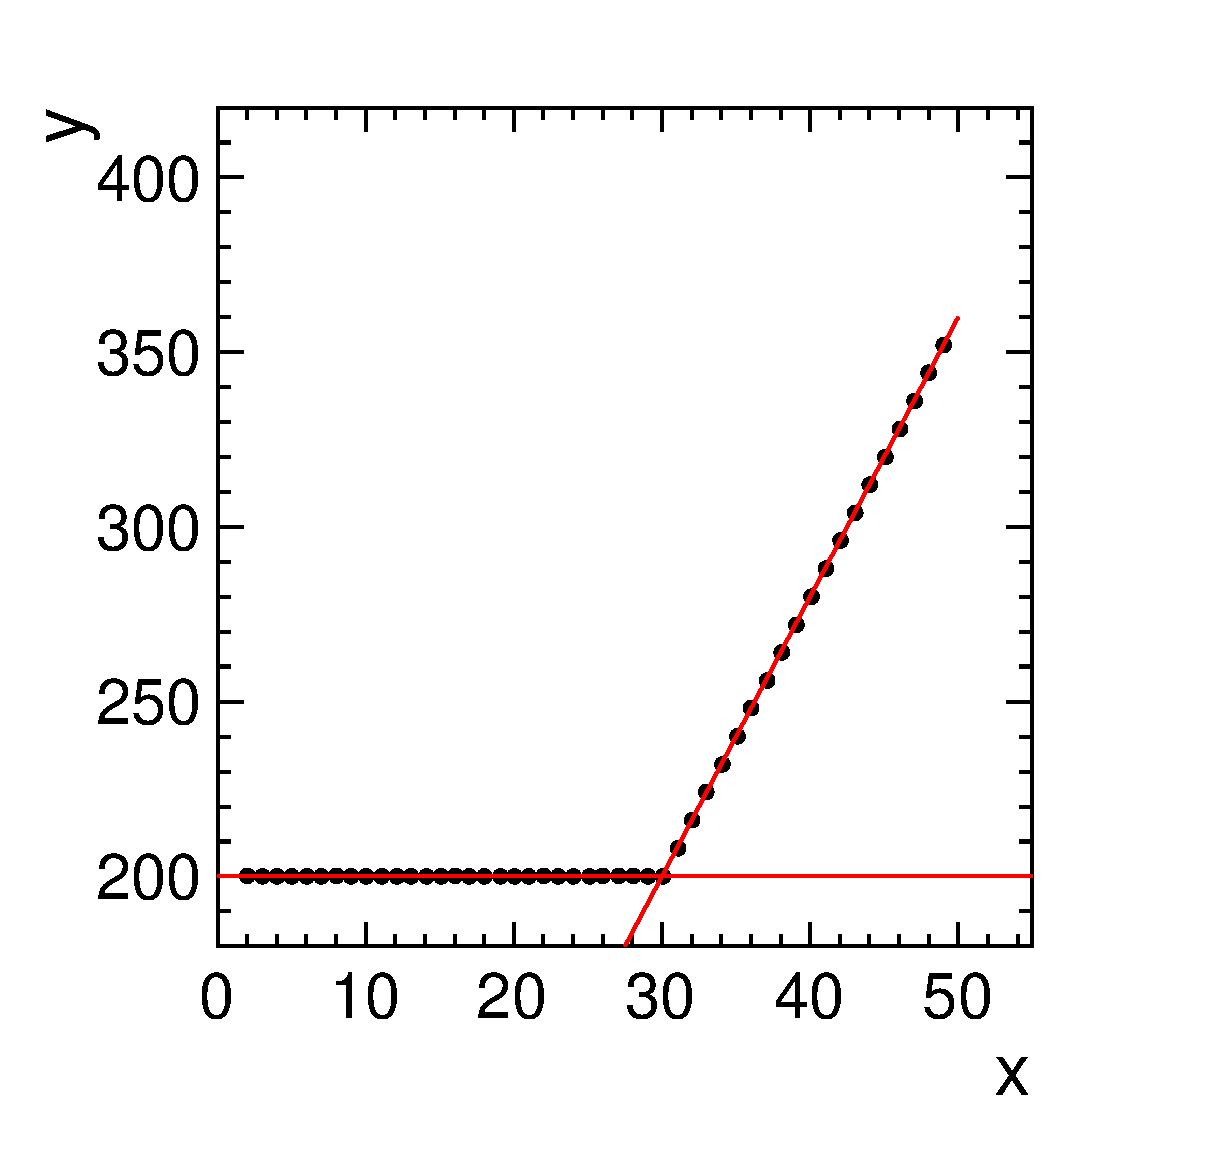
\includegraphics[width=35mm]{fig/hmap_fit.eps}
%    \end{center}
%    \caption{Two lines found with hough transform method}
%    \label{hmap_fit}
%  \end{minipage}
%\end{figure}


%\subsubsection{Chi2 method}

$\chi^{2}$ method is the algorithm to 
Identify the kaon stopped point as  the point which rapidly increase fit $\chi^{2}$ to straight line.
\begin{itemize}
\item Starting from the most upstream hit in the cluster, fit the hits to straight line (Kaon track)
\item Find the point which rapidly increase fit $\chi^{2}$ to straight line.
\item Starting from the most downstream hit in the cluster, fit the hits to straight line (Muon track)
\item Find the point which rapidly increase fit $\chi^{2}$ to straight line.
\item Kaon stopped point is identified as the hit with maximum charge and around the intersection of the two lines.
\end{itemize}

Figure \ref{KsomeQuantities} shows Data and MC comparison for signal hit charge, signal width, decay point and total particle charge distribution.
Data of signal charge and signal width are consistent with MC one in error by less than two $\%$ and data of cluster charge and primary charge are consistent with  
MC one in error by less than five $\%$.

%Figure \ref{cq27_hough} shows signal hit charge distribution of restricted channel 27. 
%As shown in figure \ref{cq27_hough}, signal charge have two peaks at 300 and 500 ADCus.
%Because two peaks has correlation of $\Delta$TOF, possible assumption of the cause is that beam line were bipolarrized and the beam didn't pass in the center of the detector.
%So, we use only the event that signal charge of restricted channel 27 is less than 350.
Figure \ref{RangeVsHit_hough} shows signal hit charge distribution in different distance from the stopped point.
Data and MC are in good agreement.

\begin{figure}[htbp]
  \begin{center}
    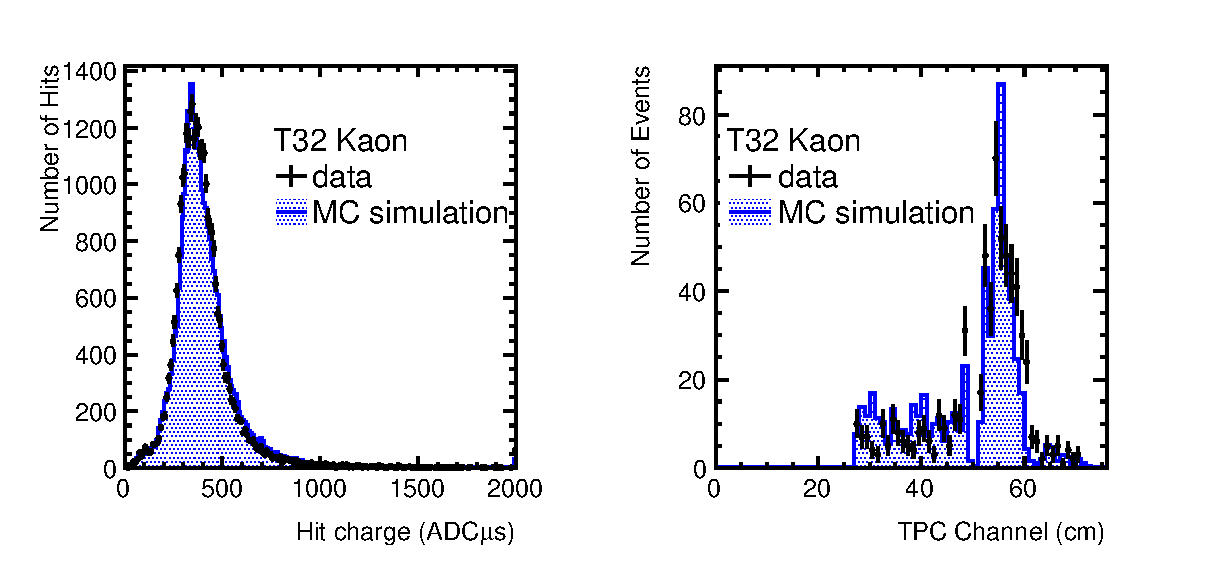
\includegraphics[width=1.0\hsize]{fig/Kaon1.eps}
  \end{center}    
    \caption{Data-MC comparison for hit charge, hit sigma, cluster charge, primary particle charge}
    \label{KsomeQuantities}
\end{figure}

%\begin{figure}[!htb]
%  \begin{center}
%    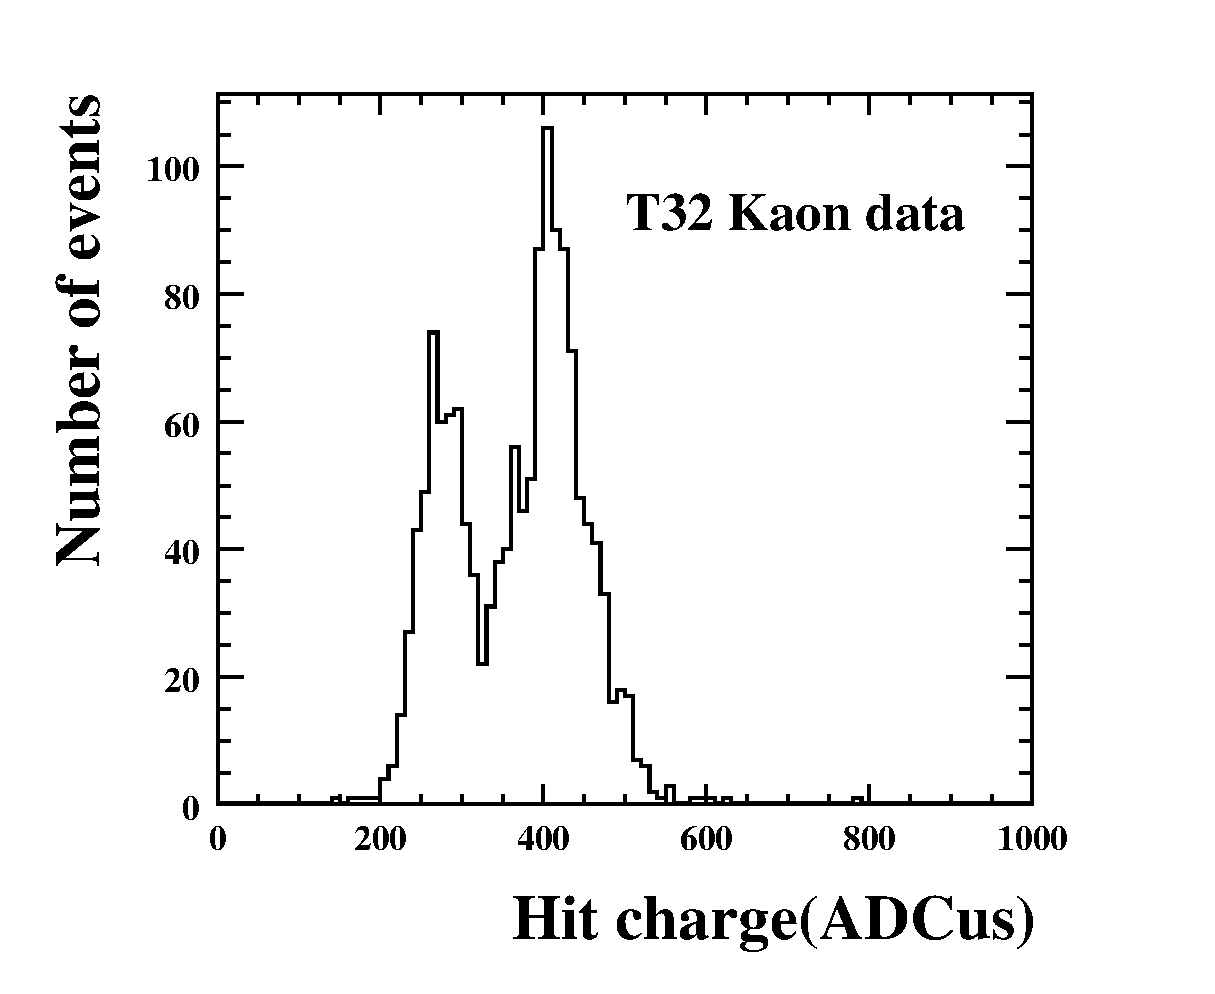
\includegraphics[width=70mm]{fig/ch27distribution.eps}
%  \end{center}
%  \label{cq27_hough}
%  \caption{Hit charge in channel 27}
%\end{figure}

\begin{figure}[!htb]
  \begin{center}
    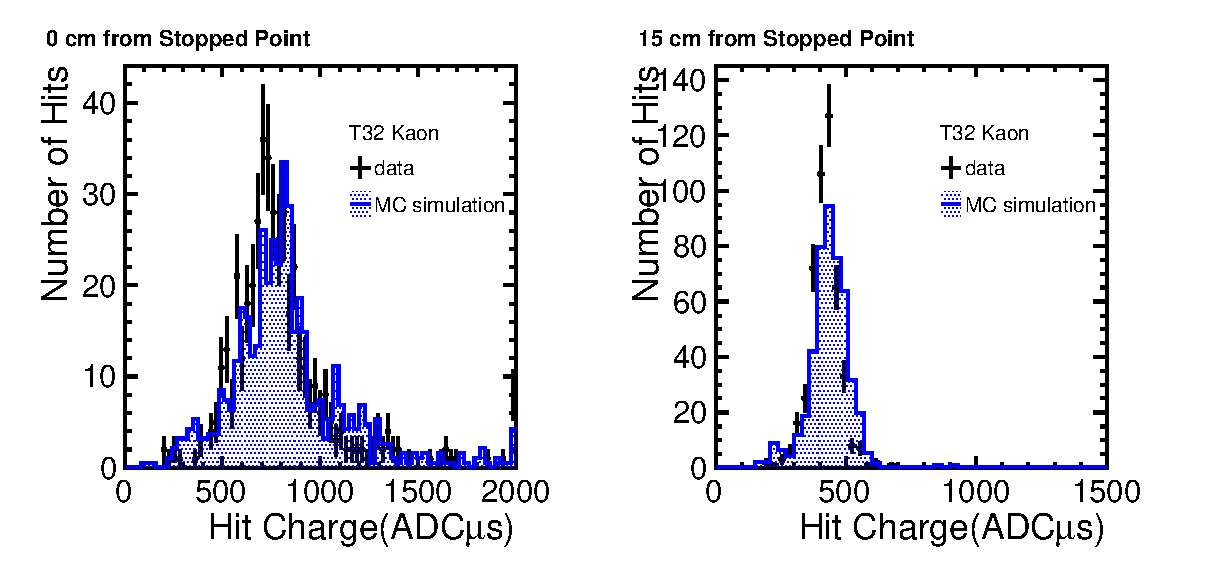
\includegraphics[width=1.0\hsize]{fig/Kaon2.eps}
  \end{center}
  \caption{Data-MC comparison for hit charge distribution in different distance from the stopped point(top left:decay point,top light:decay point-5cm,bottom left:decay point-10cm,decay point-15cm)}
  \label{RangeVsHit_hough}
\end{figure}

%As shown in figure \ref{RangeVsHit_hough}, 
Figure \ref{RangeVsHitRatio_hough} shows data/MC ratio of signal hit charge distribution in different distance from the stopped point.
Data of signal charge in different distance from stopped point are consistent with MC one with in 5$\%$.

%\begin{figure}[htb]
%  \begin{center}
%    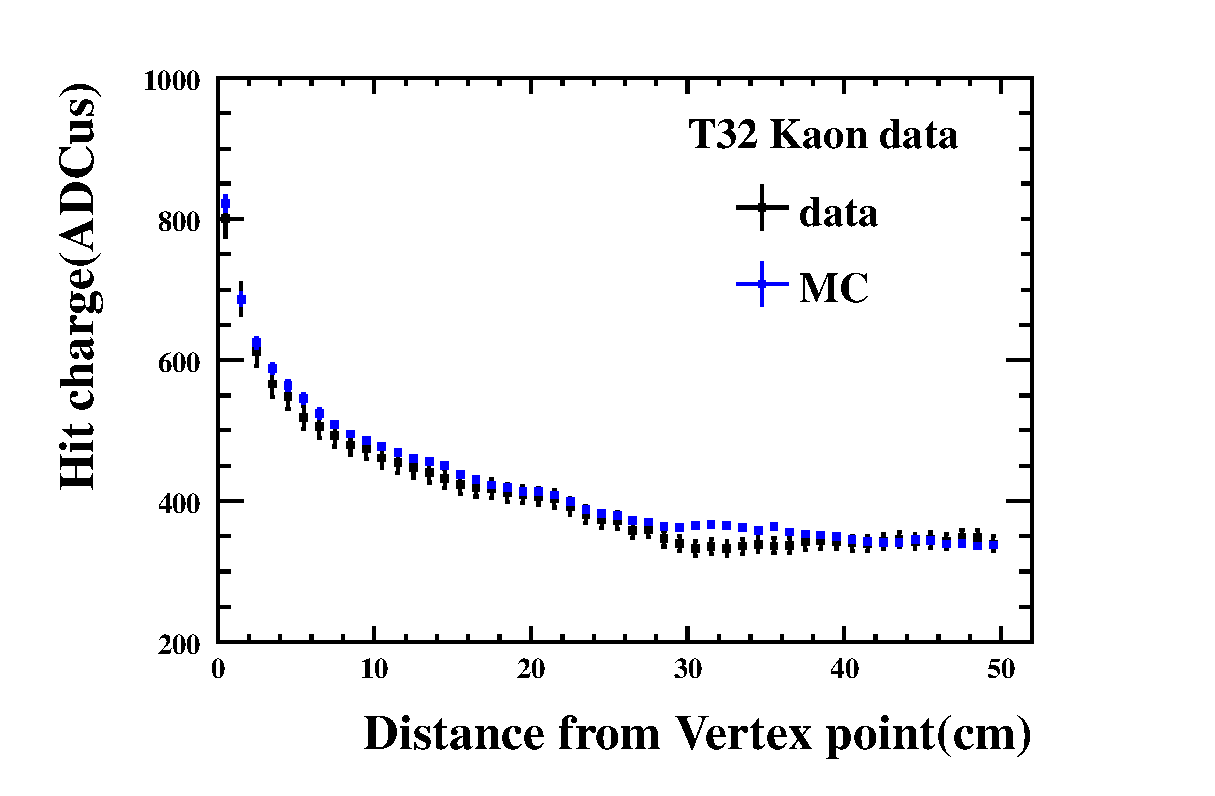
\includegraphics[width=1.0\hsize]{fig/RangeVsHitfabs_wcut_hough.eps}
 %   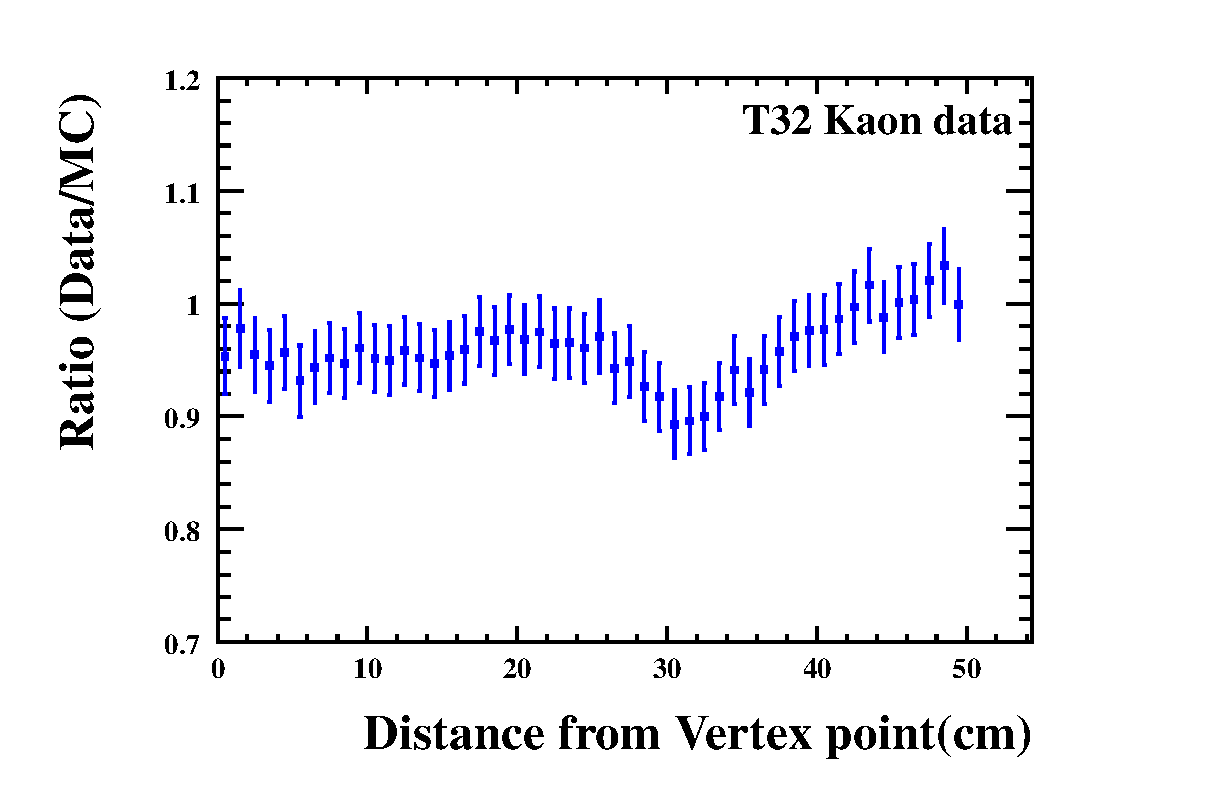
\includegraphics[width=0.8\hsize]{fig/RangeVsHitRatio_wcut_hough.eps}
%  \end{center}
%  \caption{Top plot shows Data-MC comparison for hit charge distribution in different distance from the stopped point.
%    Bottom plot shows Data/MC ratio for hit charge distribution in different distance from the stopped point}
%  \label{RangeVsHitfabs_hough}
%  \label{RangeVsHitRatio_hough}
%\end{figure}



